\documentclass[a4paper, 10pt]{article}
\usepackage{graphicx}
\usepackage[english]{babel}

\author{Andreas Precht Poulsen & Christian Rostrup Nielsen}

\begin{document}

\section{Vision}
The purpose of this program is to make a calendar that gives a graphical overview of the daily tasks.

\section{Use Cases}

\begin{itemize}
\item \textbf{UC1: Manipulating information}
	\begin{itemize}
	\item \textbf{Primary actor:}
		\\The user
	\item \textbf{Stakeholders and interests:}
		\\The user: Wants to manipulate information in the calendar
	\item \textbf{Precondition:}
		\\The user is logged in to the system
	\item \textbf{Postcondition:}
		\\The changes the user made is saved in the system.
	\item \textbf{Basic flow:}
		\\The user logs in to the system and either
		\begin{itemize}
			\item a: types in a task
			\item b: edit an existing task
			\item c: deletes an existing task
		\end{itemize}
	\end{itemize}

\item \textbf{UC2: Viewing information}
	\begin{itemize}
	\item \textbf{Primary actor:}
		\\The user
	\item \textbf{Stakeholders and interests:}
		\\The user: Wants an overview of the daily or weekly tasks
	\item \textbf{Precondition:}
		\\The user is logged in to the system
	\item \textbf{Postcondition:}
		\\No changes has been made to any tasks.
	\item \textbf{Basic flow:}
		\\The user logs in to the system and either
		\begin{itemize}
			\item a: view already existing tasks, daily
			\item b: view already existing tasks, weekly
		\end{itemize}
	\end{itemize}
\end{itemize}

\section{Use Case UML Diagrams}

\includegraphics[width=\linewidth]{../Pictures/A36_Use_Case_UML_Diagram.png} 

\section{Glossary}
Task - Is used to describe any event that is added to the calendar

\section{Supplementary Requirements}
The program must...
\begin{itemize}
\item \textbf{Functionality}
	\\support the tasks that a user needs in order to sustain an up to date calendar, that can be used to view task throughout the weeks. Furthermore it should not be possible for different users to view other users tasks.
\item \textbf{Usability}
	\\be easy to use, enabling almost anyone to use it without much hassle.
\item \textbf{Reliability}
	\\be available at all times, as the need for the calendar can emerge at any given time.
\item \textbf{Performance}
	\\not use unnecessary resources and should be able to show tasks for a given period within seconds of request.
\item \textbf{Supportability}
	\\be maintainable by other programmers than the original. Additionally it must be possible to extend the program with functionality. The program should be able to run on most modern devices.
\end{itemize}

\section{Domain Model}
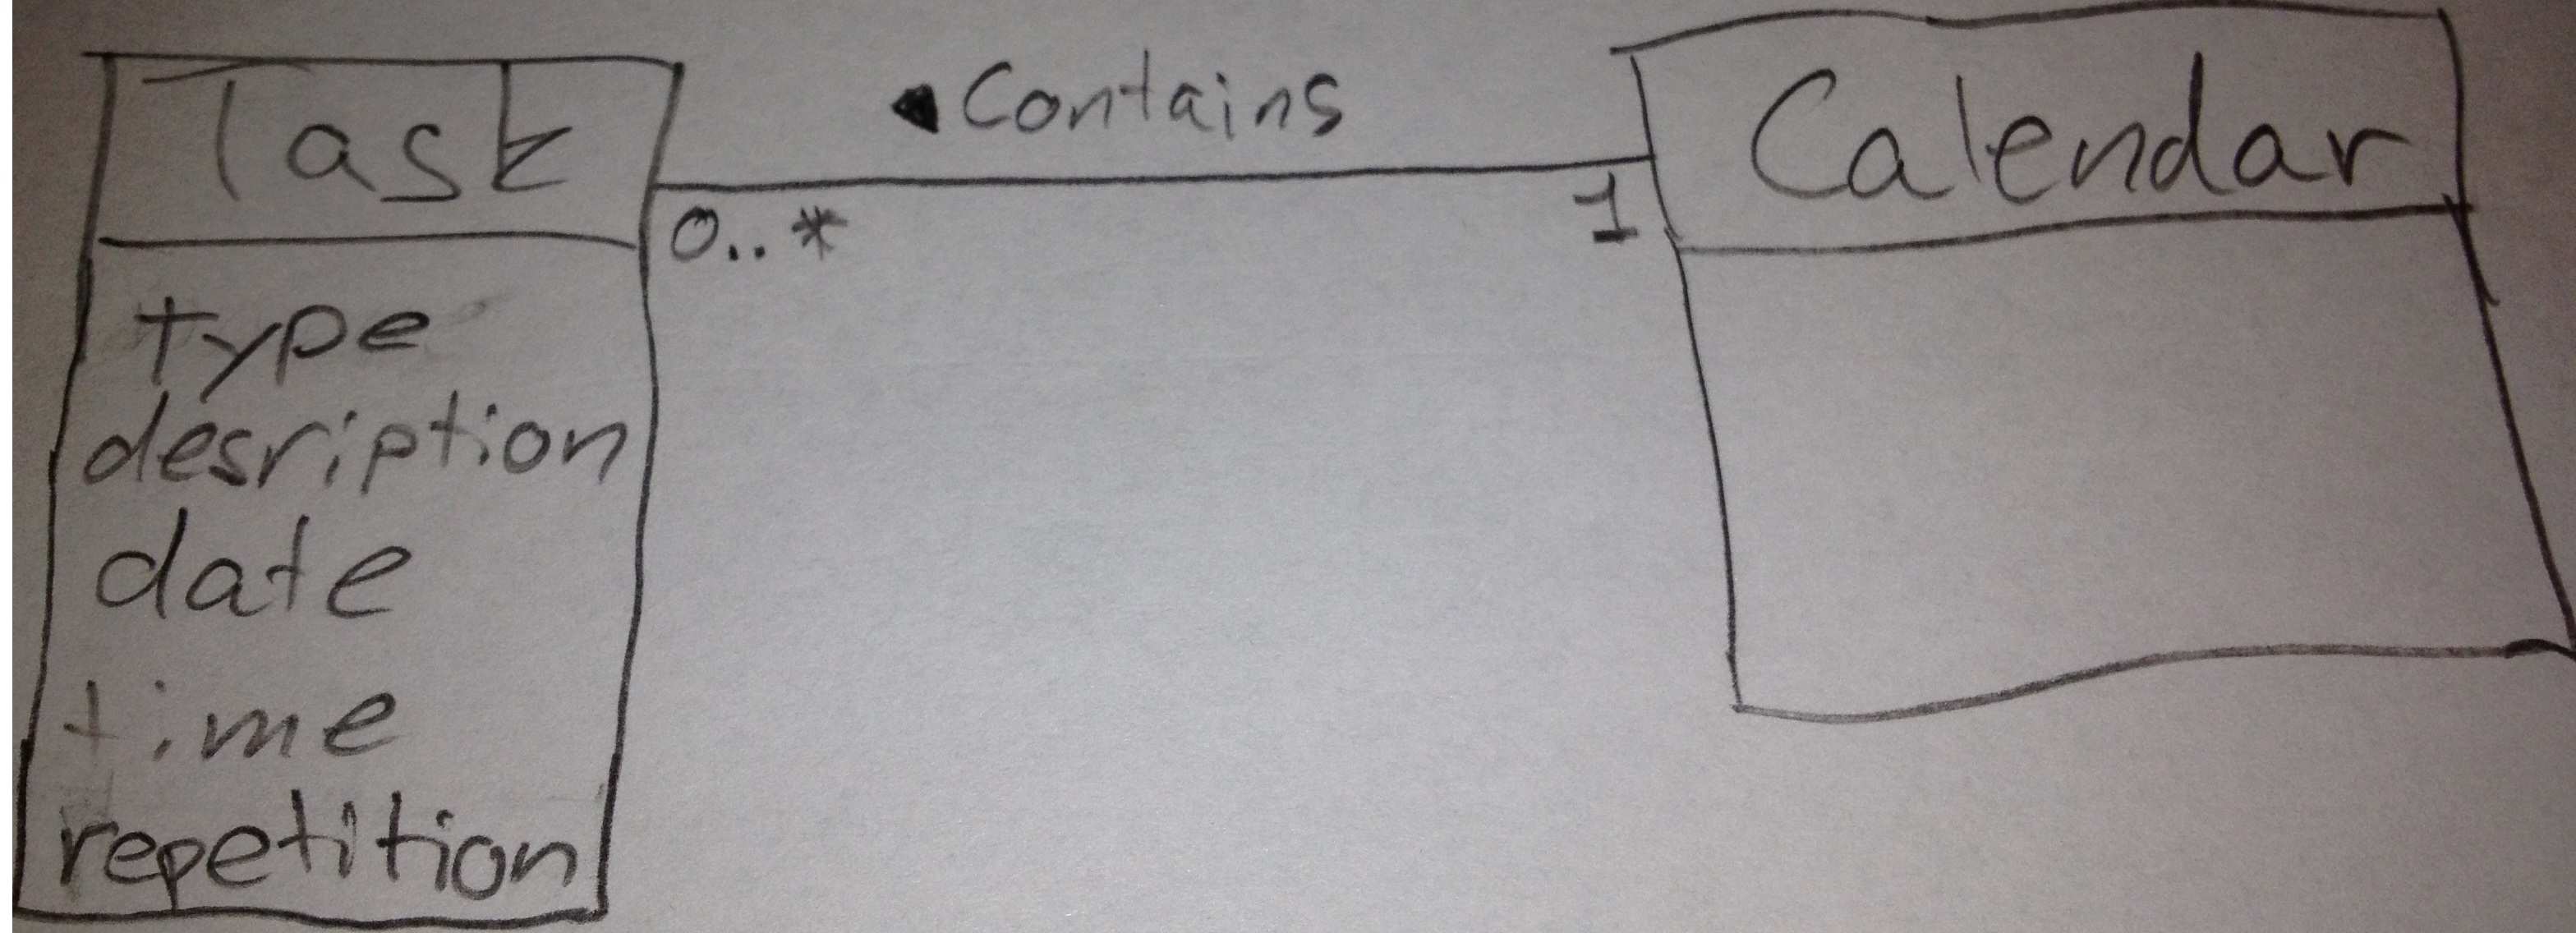
\includegraphics[width=\linewidth]{../Pictures/A38_Domain_Model.jpg} 

\section{System Sequence Diagram}
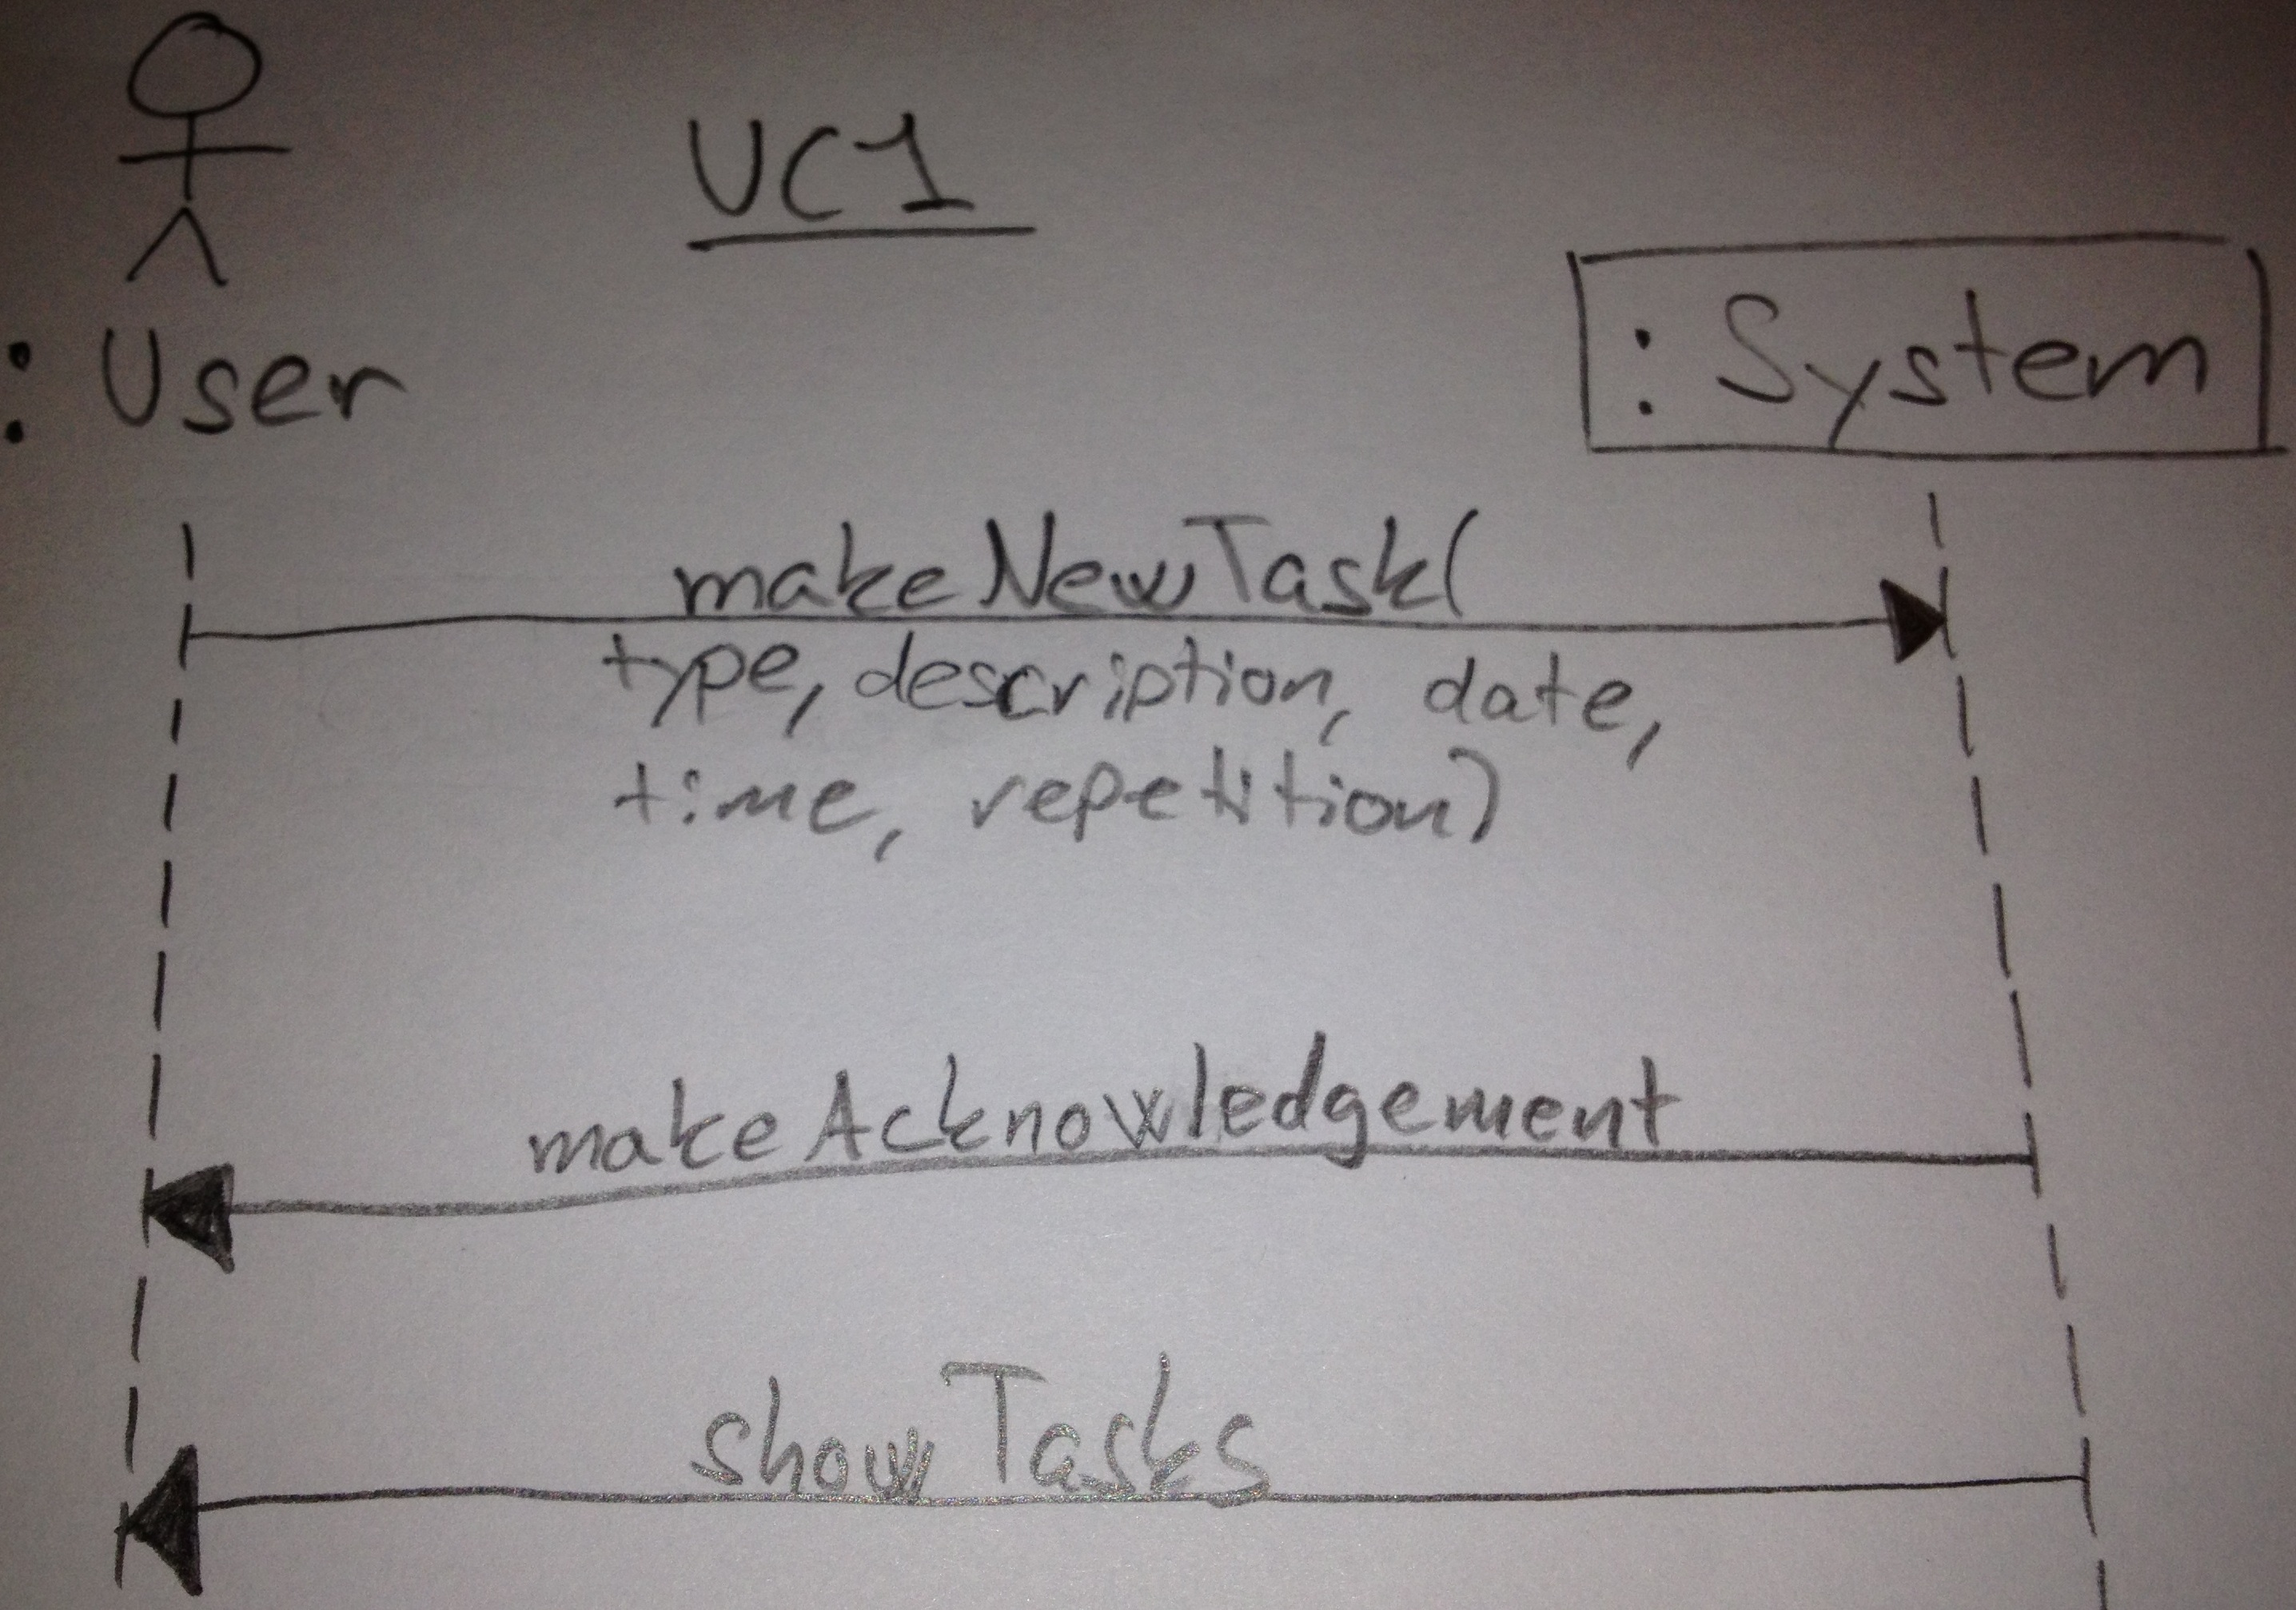
\includegraphics[width=\linewidth]{../Pictures/A38_SSD_UC1.jpg} 

\section{Operations Contract}
\begin{description}
\item[\large Contract OC1: makeNewTask] \hfill \\
\begin{tabular}{ r l }
	\textbf{Operation:} & makeNewTask(type, description, date, time, repetition) \\
	\textbf{Cross References:} & Use Cases: UC1 \\
	\textbf{Preconditions:} & The user is logged in. \\
	\textbf{Postconditions:} & The new task is saved in the system.
\end{tabular}
\end{description}

\section{Discussion of software attributes}
Due to the fact that many people store personal information and personal tasks, like an appointment at the Doctor's, we would like to make our system as secure as possible while still retaining an acceptable performance. \\
The availability (or uptime) of our system is quite crucial since a calendar you can't access isn't of much use.

\section{UML Package Diagram}
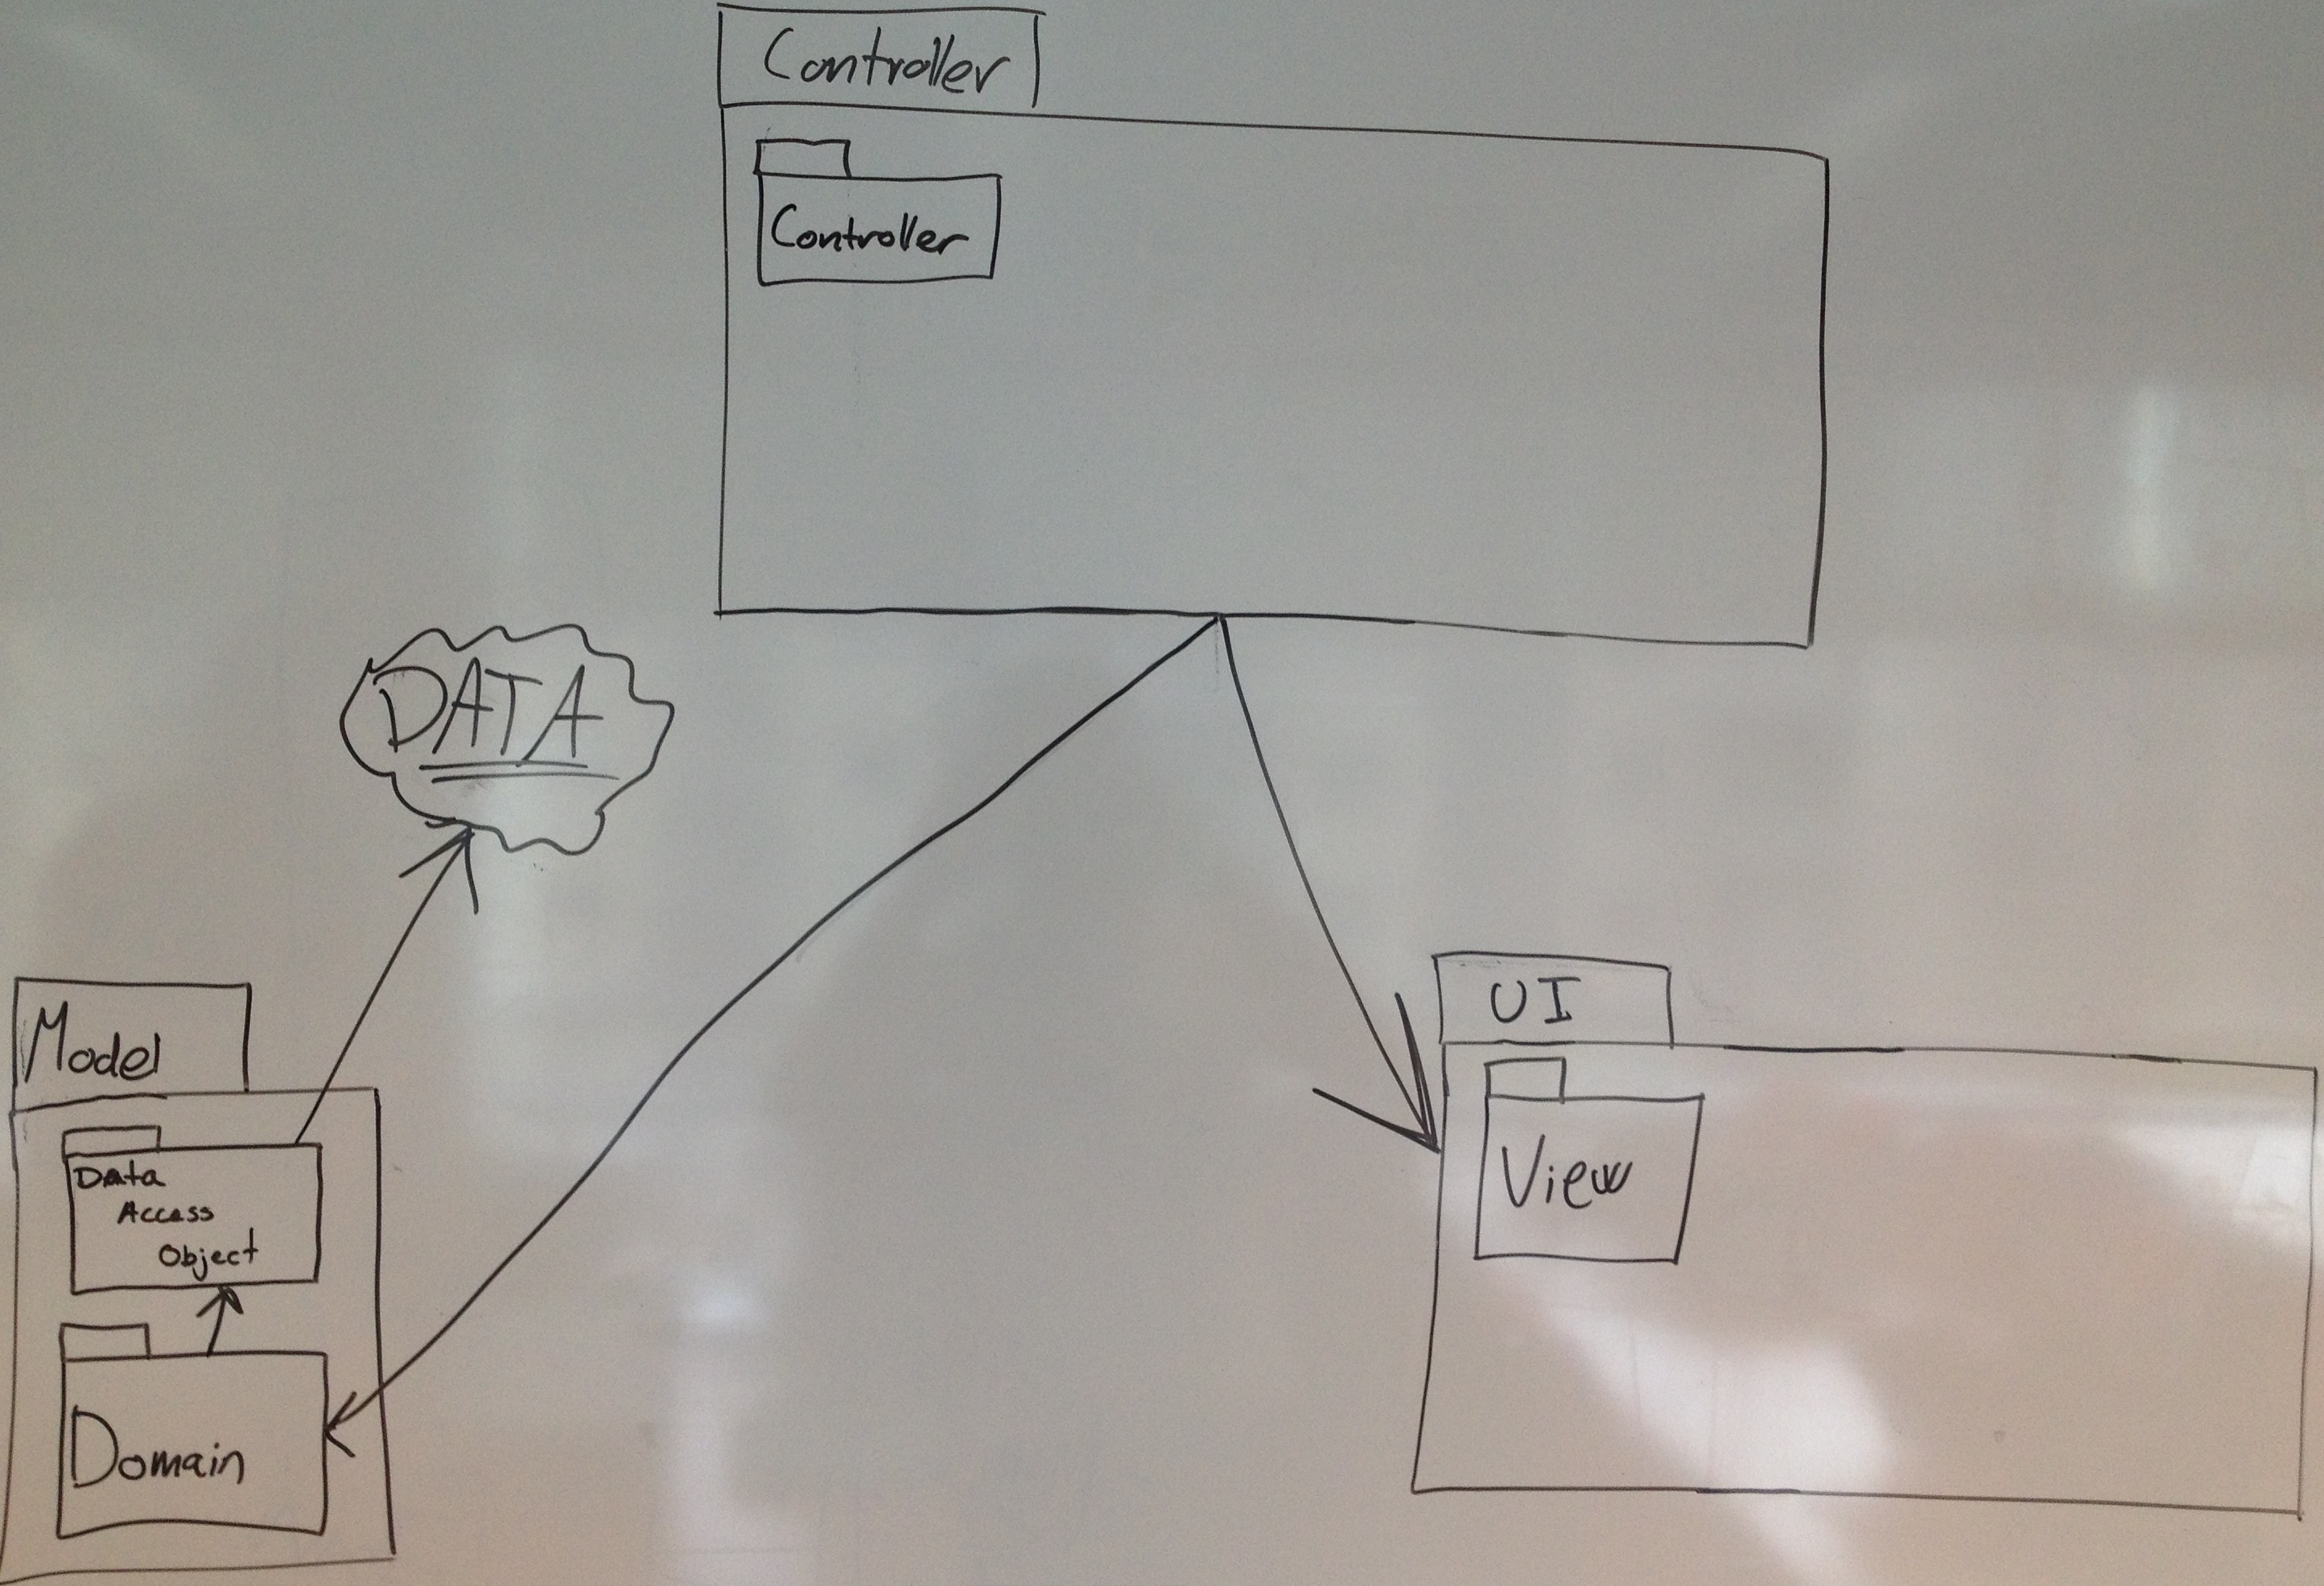
\includegraphics[width=\linewidth]{../Pictures/UML_Package_Diagram.jpg}

\section{Interaction Diagrams}
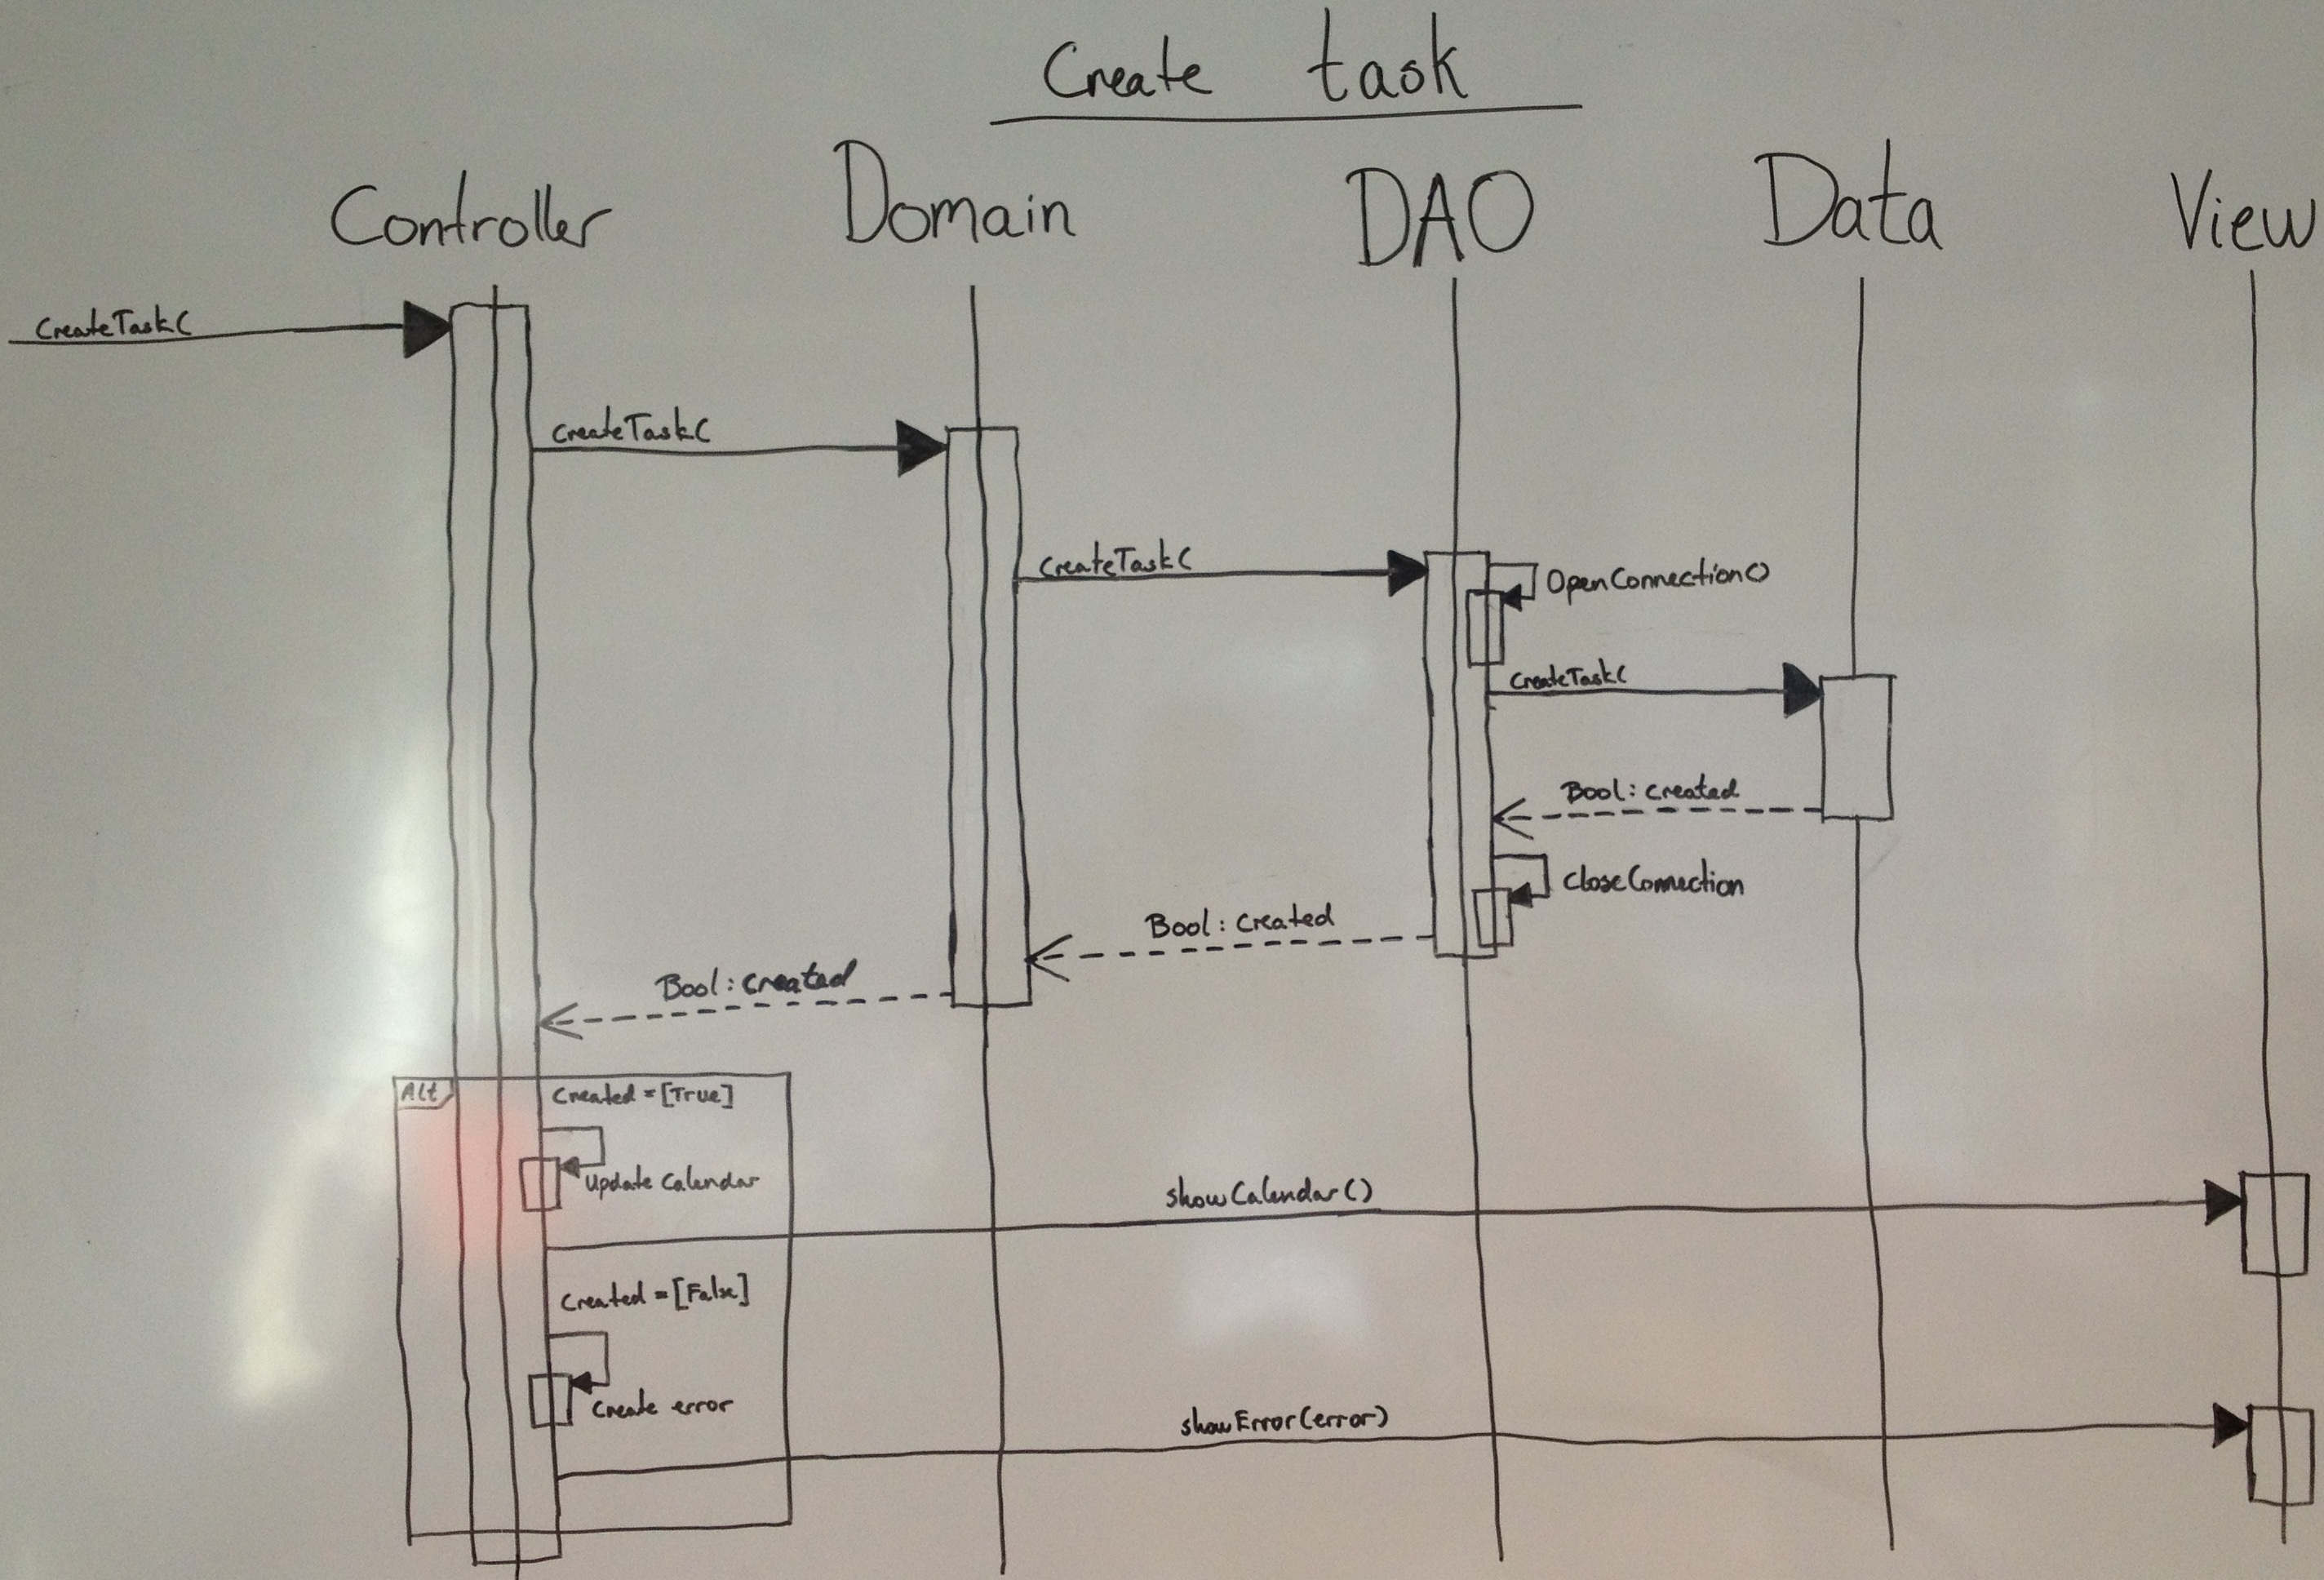
\includegraphics[width=\linewidth]{../Pictures/Interaction_Diagram_Create_Task.jpg}
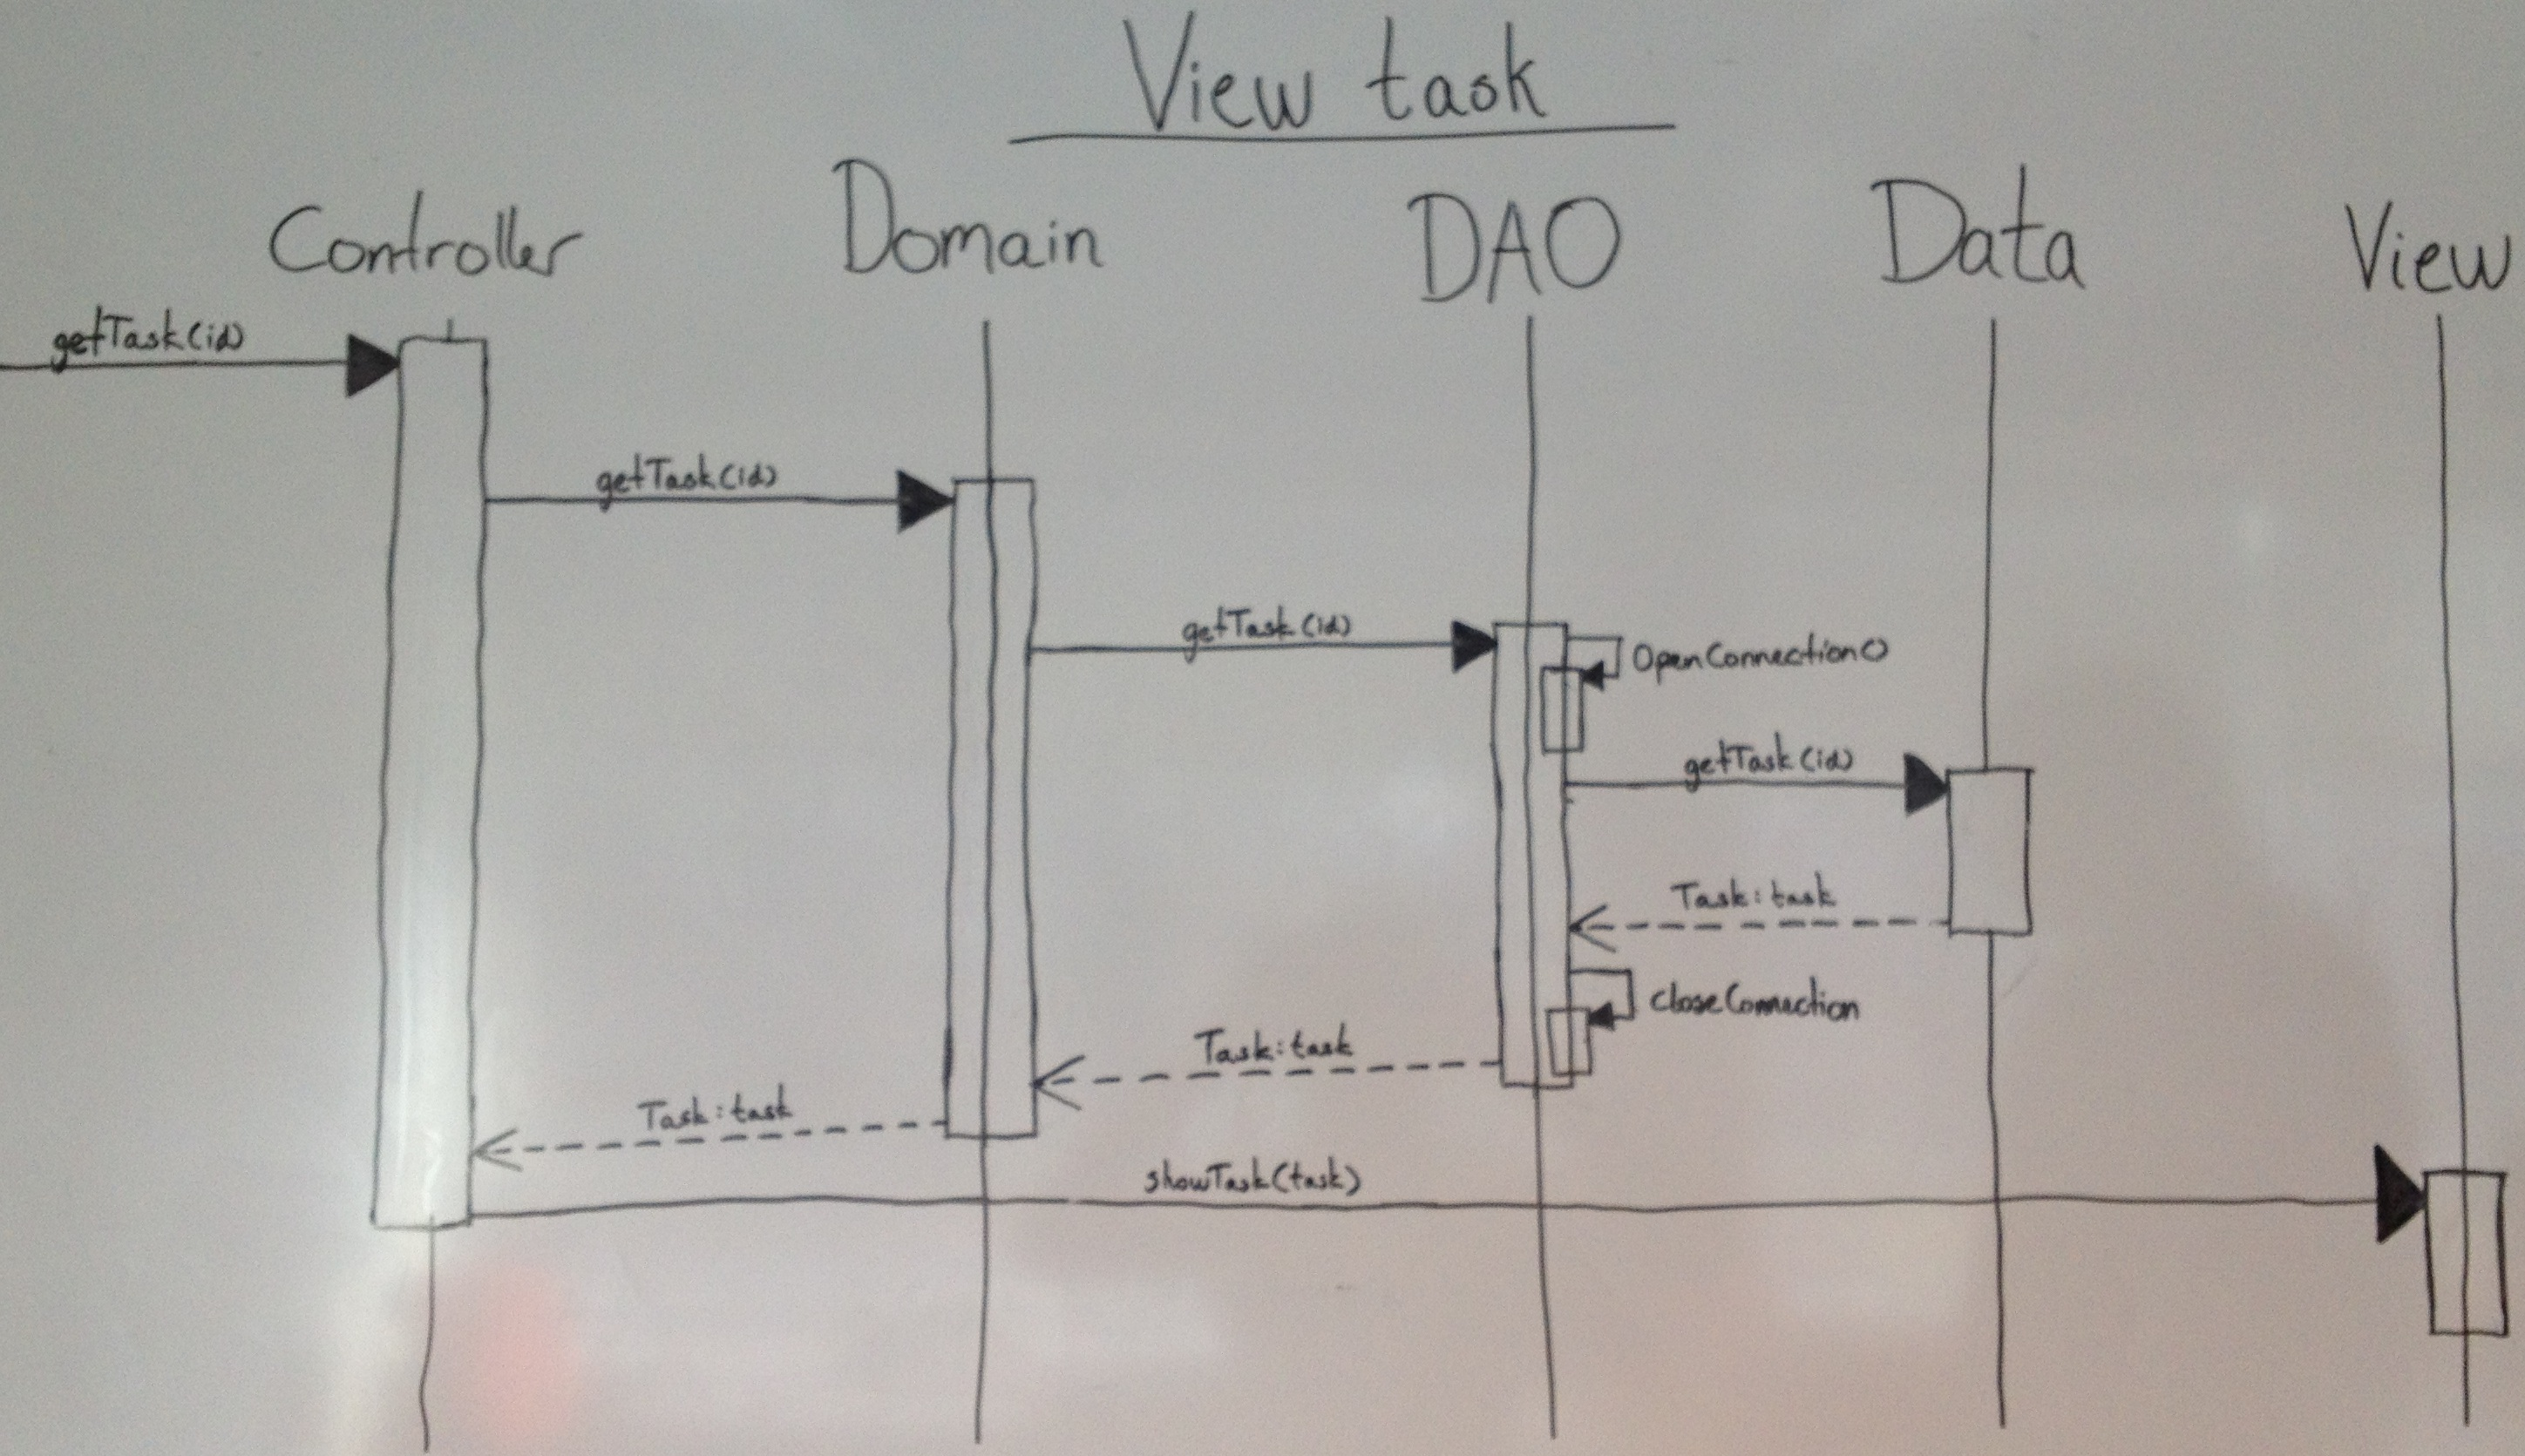
\includegraphics[width=\linewidth]{../Pictures/Interaction_Diagram_View_Task.jpg}

\section{Design Class Diagram}
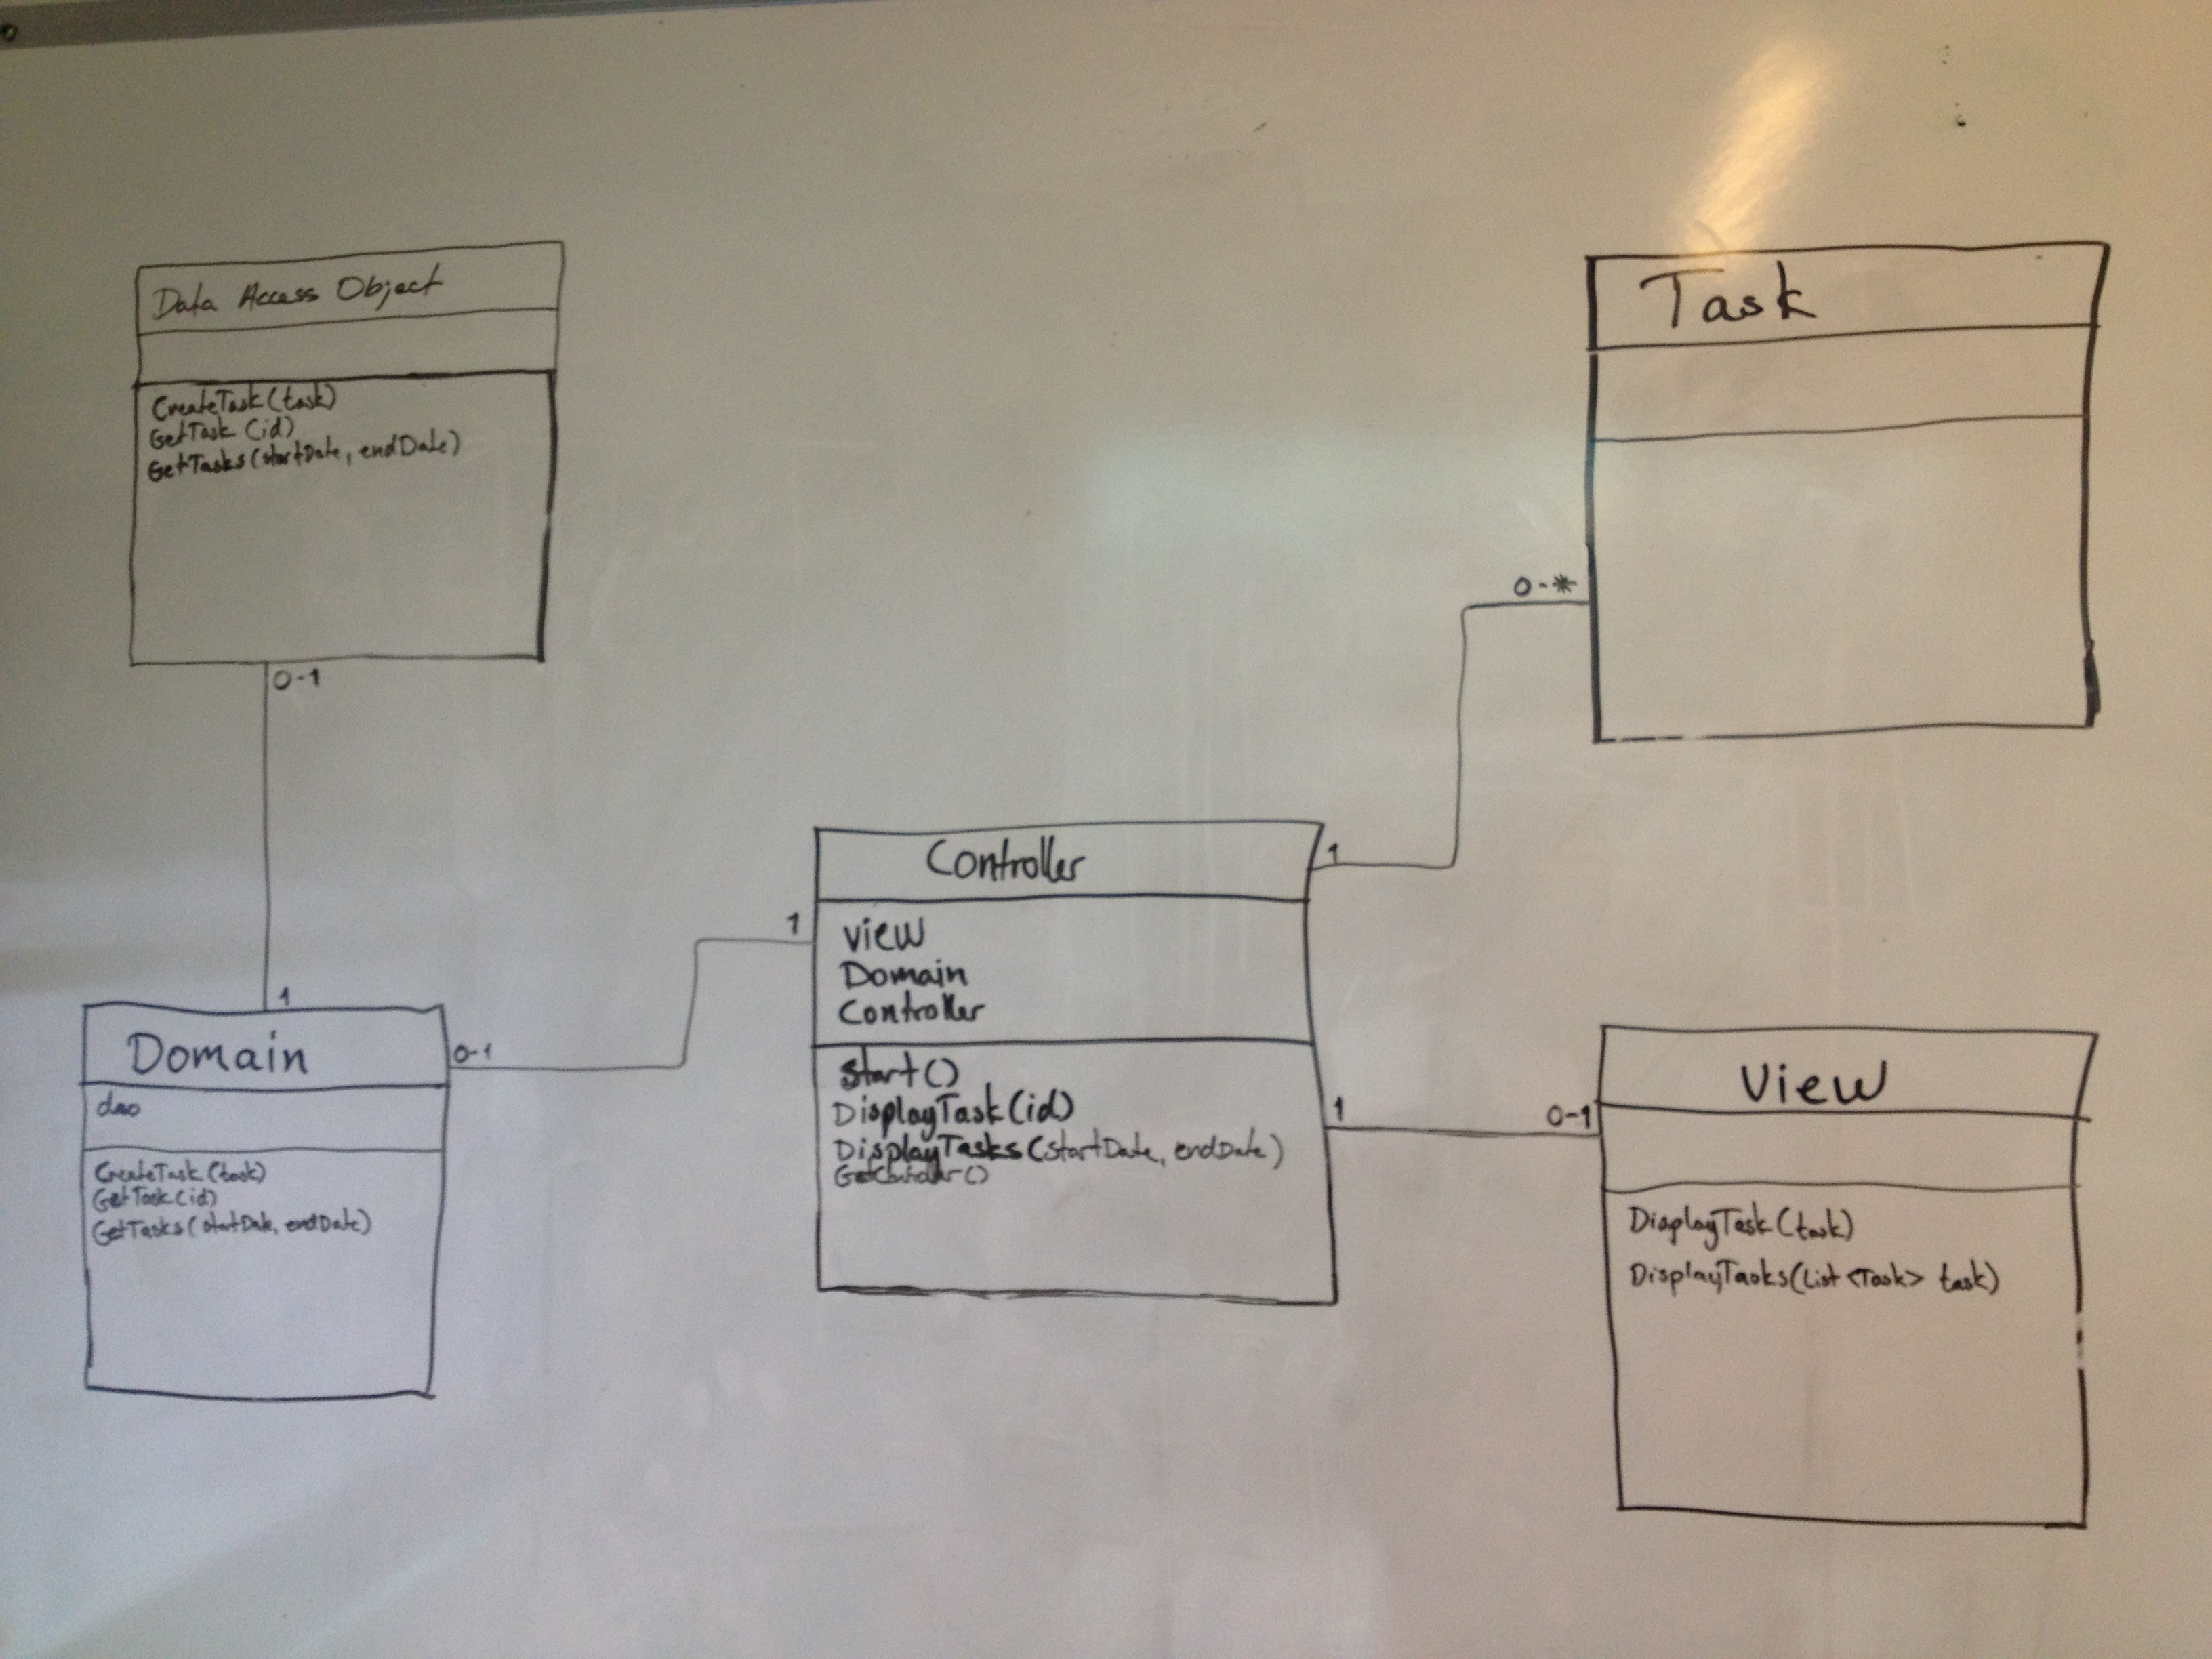
\includegraphics[width=\linewidth]{../Pictures/Design_Class_Diagram.jpg}

\section{Revision History}
\begin{tabular}{ | c | c | p{6cm} | p{3cm} | }
\hline
\textbf{Version} & \textbf{Date} & \textbf{Description} & \textbf{Author}
\\ \hline
1 & 20. sep 2012 & - Added: Vision, Use Cases, Use Case UML Diagrams, Glossary \& Supplementary Requirements - Changes: None & Andreas Precht \& Christian Rostrup
\\ \hline
2 & 02. oct 2012 & - Added: Discussion, Revision History, UML Package Diagram \& Interaction Diagrams - Changes: Operation Contract& Andreas Precht \& Christian Rostrup
\\ \hline
3 & 09 oct 2012 & - Added: Design Class Diagram & Andreas Precht \& Christian Rostrup
\end{tabular}



\end{document}